\documentclass{article}
\usepackage{tikz}

\begin{document}

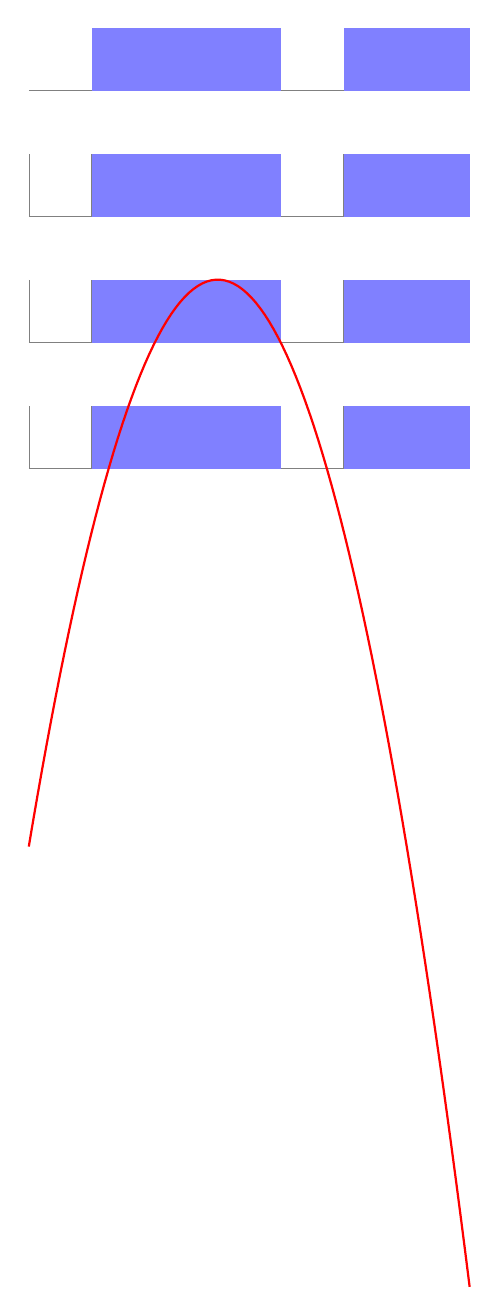
\begin{tikzpicture}[scale=0.8]
    % Draw the grid
    \draw[help lines] (0,0) grid (7,7);
    
    % Fill the cells with different colors
    \fill[blue!50] (1,1) rectangle (2,2);
    \fill[blue!50] (2,1) rectangle (3,2);
    \fill[blue!50] (3,1) rectangle (4,2);
    \fill[blue!50] (1,3) rectangle (2,4);
    \fill[blue!50] (2,3) rectangle (3,4);
    \fill[blue!50] (3,3) rectangle (4,4);
    \fill[blue!50] (1,5) rectangle (2,6);
    \fill[blue!50] (2,5) rectangle (3,6);
    \fill[blue!50] (3,5) rectangle (4,6);
    \fill[blue!50] (1,7) rectangle (2,8);
    \fill[blue!50] (2,7) rectangle (3,8);
    \fill[blue!50] (3,7) rectangle (4,8);
    \fill[blue!50] (5,1) rectangle (6,2);
    \fill[blue!50] (6,1) rectangle (7,2);
    \fill[blue!50] (5,3) rectangle (6,4);
    \fill[blue!50] (6,3) rectangle (7,4);
    \fill[blue!50] (5,5) rectangle (6,6);
    \fill[blue!50] (6,5) rectangle (7,6);
    \fill[blue!50] (5,7) rectangle (6,8);
    \fill[blue!50] (6,7) rectangle (7,8);
    \fill[white] (0,0) rectangle (1,1);
    \fill[white] (0,2) rectangle (1,3);
    \fill[white] (0,4) rectangle (1,5);
    \fill[white] (0,6) rectangle (1,7);
    \fill[white] (1,0) rectangle (2,1);
    \fill[white] (1,2) rectangle (2,3);
    \fill[white] (1,4) rectangle (2,5);
    \fill[white] (1,6) rectangle (2,7);
    \fill[white] (2,0) rectangle (3,1);
    \fill[white] (2,2) rectangle (3,3);
    \fill[white] (2,4) rectangle (3,5);
    \fill[white] (2,6) rectangle (3,7);
    \fill[white] (3,0) rectangle (4,1);
    \fill[white] (3,2) rectangle (4,3);
    \fill[white] (3,4) rectangle (4,5);
    \fill[white] (3,6) rectangle (4,7);
    \fill[white] (4,0) rectangle (5,1);
    \fill[white] (4,2) rectangle (5,3);
    \fill[white] (4,4) rectangle (5,5);
    \fill[white] (4,6) rectangle (5,7);
    \fill[white] (5,0) rectangle (6,1);
    \fill[white] (5,2) rectangle (6,3);
    \fill[white] (5,4) rectangle (6,5);
    \fill[white] (5,6) rectangle (6,7);
    \fill[white] (6,0) rectangle (7,1);
    \fill[white] (6,2) rectangle (7,3);
    \fill[white] (6,4) rectangle (7,5);
    \fill[white] (6,6) rectangle (7,7);
    
    % Draw the red curve
    \draw[red, thick, domain=0:7, samples=100] plot (\x, {-(\x-3)^2 + 4});
\end{tikzpicture}

\end{document}